% BEGIN LICENSE BLOCK
% Version: CMPL 1.1
%
% The contents of this file are subject to the Cisco-style Mozilla Public
% License Version 1.1 (the "License"); you may not use this file except
% in compliance with the License.  You may obtain a copy of the License
% at www.eclipse-clp.org/license.
%
% Software distributed under the License is distributed on an "AS IS"
% basis, WITHOUT WARRANTY OF ANY KIND, either express or implied.  See
% the License for the specific language governing rights and limitations
% under the License.
%
% The Original Code is  The ECLiPSe Constraint Logic Programming System.
% The Initial Developer of the Original Code is  Cisco Systems, Inc.
% Portions created by the Initial Developer are
% Copyright (C) 2006 Cisco Systems, Inc.  All Rights Reserved.
%
% Contributor(s):
%
% END LICENSE BLOCK
%----------------------------------------------------------------------
\chapter{Development Support Tools\label{chapdevelsupport}}
%HEVEA\cutdef[1]{section}
\index{program analysis}
%----------------------------------------------------------------------

This chapter describes some of the tools and libraries provided by
\eclipse{} that assist in program development and the analysis of
program runtime behaviour.
\index{performance}\index{optimisation}\index{profiling}
\index{code coverage}
%----------------------------------------------------------------------
\section{Available Tools and Libraries}
%----------------------------------------------------------------------

\eclipse{} provides a number of different tools and libraries to assist
the programmer with program development:

\begin{quote}
\begin{description}
  \item[Document]\libidx{document}
    Tools for generating documentation from ECLiPSe sources.
  \item[Lint]\libidx{lint}
    Generates warning messages for dubious programming
    constructs and violation of naming conventions for an ECLiPSe source
    module or file.
  \item[Pretty_printer]\libidx{pretty_printer}
    Tools for pretty-printing a file in different formats.
  \item[Xref]\libidx{xref}
    Enables the analysis of an ECLiPSe source module or
    file for the construction of a predicate call graph.
\end{description}
\end{quote}

In addition, \eclipse{} provides several tools that aid in the
understanding of a programs runtime behaviour:

\begin{quote}
\begin{description}
\item[Coverage] Records the frequency at which various parts of the
program are executed.
\item[Debugger] Provides a low level view of program
activity. Chapter~\ref{chapdebug} presents a comprehensive
look at debugging of \eclipse{} programs.
\item[Display matrix] Shows the values of given terms in a graphical
window. Chapter~\ref{chaptkeclipse} discusses the use of this tool.
\item[Mode Analyser] Collects statistics about the invocation modes of
predicates within a running program in order to assist in the generation of
compiler invocation mode directives.
\item[Port Profiler] Collects statistics about the running program in terms
of box model port counters.
\item[Timing Profiler] Samples the running program at regular intervals to
give a statistical summary of where the execution time is spent.
\item[Visualisation framework] A graphical environment for the
visualisation of search and propagation in constraint programs.
The \about{Visualisation Tools Manual} discusses the use of this
environment.
\end{description}
\end{quote}

This section focuses on the program development libraries and two
complementary runtime analysis tools, the \libspec{profiler} and the
\libspec{coverage} library.
Throughout this chapter, the use of each of the tools is demonstrated
on the following \examplename{n-queens} code:
\begin{quote}
\begin{verbatim}
:- module(queen).
:- export queen/2.

queen(Data, Out) :-
        qperm(Data, Out),
        safe(Out).

qperm([], []).
qperm([X|Y], [U|V]) :-
        qdelete(U, X, Y, Z),
        qperm(Z, V).

qdelete(A, A, L, L).
qdelete(X, A, [H|T], [A|R]) :-
        qdelete(X, H, T, R).

safe([]).
safe([N|L]) :-
        nodiag(L, N, 1),
        safe(L).

nodiag([], _, _).
nodiag([N|L], B, D) :-
        D =\= N - B,
        D =\= B - N,
        D1 is D + 1,
        nodiag(L, B, D1).
\end{verbatim}
\end{quote}

%----------------------------------------------------------------------
\section{Heuristic Program Checker}
%----------------------------------------------------------------------

The Heuristic Program Checking tool generates warning messages for
dubious programming constructs and violation of naming conventions for
an ECLiPSe source module or file. It is loaded as follows:

\begin{quote}
\begin{verbatim}
:- lib(lint).
\end{verbatim}
\end{quote}

The heuristic rules currently enforced are based on the style guide of
Appendix \ref{styleguide}. These rules are somewhat limited in scope. The
library
is distributed as source and serves to provide a framework for the
addition of a more comprehensive set of rules that are tailored to each
individual developer.

Consider the following typographic mistakes in the \examplename{n-queens}
example:

\begin{quote}
\begin{verbatim}
queen(Data, Out) :-
        qperm(Datas, Out),
        safe(Out).

n0diag([], _, _).
\end{verbatim}
\end{quote}

The tool is invoked using the
\bipref{lint/1}{../bips/lib/lint/lint-1.html} predicate with the source
file specified as an atom or string:

\begin{quote}
\begin{verbatim}
?- lint(queen).

--- File /tmp/queen.ecl, line 4:
Singleton variables: [Data, Datas]

--- File /tmp/queen.ecl, line 22:
Questionable predicate name: n0diag

Yes (0.01s cpu)
\end{verbatim}
\end{quote}

The checker identifies \notation{Data} and \notation{Datas} as being singleton
variables
and is dubious of the \notation{n0diag} predicate name. Both are the result of
programmer error, \notation{Datas} should read \notation{Data} and
\notation{n0diag}
as \notation{nodiag}. The \bipref{lint/2}{../bips/lib/lint/lint-2.html}
predicate allows a list of options to be specified that turn on
and off the heuristic rules.

%----------------------------------------------------------------------
\section{Document Generation Tools}
%----------------------------------------------------------------------

The document generation tools library provides a set of predicates for
the generation of documentation from \eclipse{} program sources. The
tools generate documentation by processing the
\bipref{comment/2}{../bips/kernel/directives/comment-2.html}
directives in each source file. The following is an example comment for
the \examplename{n-queens} example:

\begin{quote}
\begin{verbatim}
% comment for queen/2
:- comment(queen/2, [

    summary: "Program that solves the attacking Queens problem for
              an arbitrary number of queens.",

    index: ["NQueens Problem"],

    args: ["Data": "List modelling initial state of queens on board.",
       "Args": "Solution list of Y-coordinate of each queen on the
        board."],

    amode: queen(+,-),
    amode: queen(-,+),
    amode: queen(+,+),

    resat: yes,

    fail_if: "A solution cannot be found where all queens are safe
              from attack by every other.",

    see_also:
        [queens8/1, queensN/1],

    desc: html("The problem is to arrange a specified number of queens
           on a chessboard such that no queen attacks any other queen
           The predicate takes a list representing the initial state
           of the queens on the board, with each element representing
           a queen and its current Y-coordinate. If a solution is
           found, a list is returned specifying the safe Y-coordinate
	   for each queen.")
   ]).  % end of comment directive for queen/2
\end{verbatim}
\end{quote}

There are two pertinent predicates for document generation. The first,
\bipref{icompile/2}{../bips/lib/document/icompile-2.html} generates an
information file (with the extension \notation{.eci}) by extracting information
from a source file (whose extension is \notation{.ecl}).
The second,
\bipref{eci_to_html/3}{../bips/lib/document/eci_to_html-3.html},
processes this information file to produce readable HTML and plain text files.
By default, these files are placed in a subdirectory with the
same name as the information file, but without the extension.
The generated files are \notation{index.html}, containing a summary
description of the library, plus one HTML and one plain text file
for each predicate that was commented using a \predspec{comment/2} directive
in the source.

The following produces the \notation{queen.eci} file and a \notation{queen}
directory in the current directory. Within the queen directory reside
\notation{index.html}, \notation{queen-2.html} and \notation{queen-2.txt}:
\begin{quote}
\begin{verbatim}
?- lib(document).
document.ecl compiled traceable 83620 bytes in 0.04 seconds
Yes (0.04s cpu)

?- icompile(queen, ".").
queen.ecl  compiled traceable 1432 bytes in 0.01 seconds
/examples/queen.eci generated in 0.00 seconds.
Yes (0.01s cpu)

?- eci_to_html(queen, ".", "").
Yes (0.00s cpu)
\end{verbatim}
\end{quote}

%----------------------------------------------------------------------
\section{Cross Referencing Tool}
%----------------------------------------------------------------------

The cross referencing library \libspec{xref} analyses an ECLiPSe source
module or file and builds its predicate call graph. The graph can either
be returned in the format of \notation{lib(graph_algorithms)}, as text, or
as a graphical display.

The \bipref{xref/2}{../bips/lib/xref/xref-2.html} predicate is invoked
as \notation{xref(File,~Options)}. This generates
a call graph for the file \about{File} according to the \about{Options}
list.  The options specify the format of the graph to be generated, whether
calls to built in predicates are displayed and whether it is a caller
or callee graph:
\begin{quote}
\begin{verbatim}
?- xref:xref(queen, []).

nodiag / 3 calls:
        nodiag / 3

qdelete / 4 calls:
        qdelete / 4

qperm / 2 calls:
        qdelete / 4
        qperm / 2

queen / 2 calls:
        qperm / 2
        safe / 1

safe / 1 calls:
        nodiag / 3
        safe / 1

Yes (0.01s cpu)
?- xref:xref(queen,[builtins:on,output:daVinci]).
WARNING: module 'daVinci' does not exist, loading library...
daVinci.ecl compiled traceable 5644 bytes in 0.01 seconds
\end{verbatim}
\end{quote}

The first \notation{xref} predicate call generates a textual call graph
for the \notation{queen} module, while the second generates the
\notation{daVinci} graph illustrated in figure~\ref{xrefdavinci}.

\begin{figure}[hbt]
\begin{center}
\resizebox{0.8\textwidth}{!}{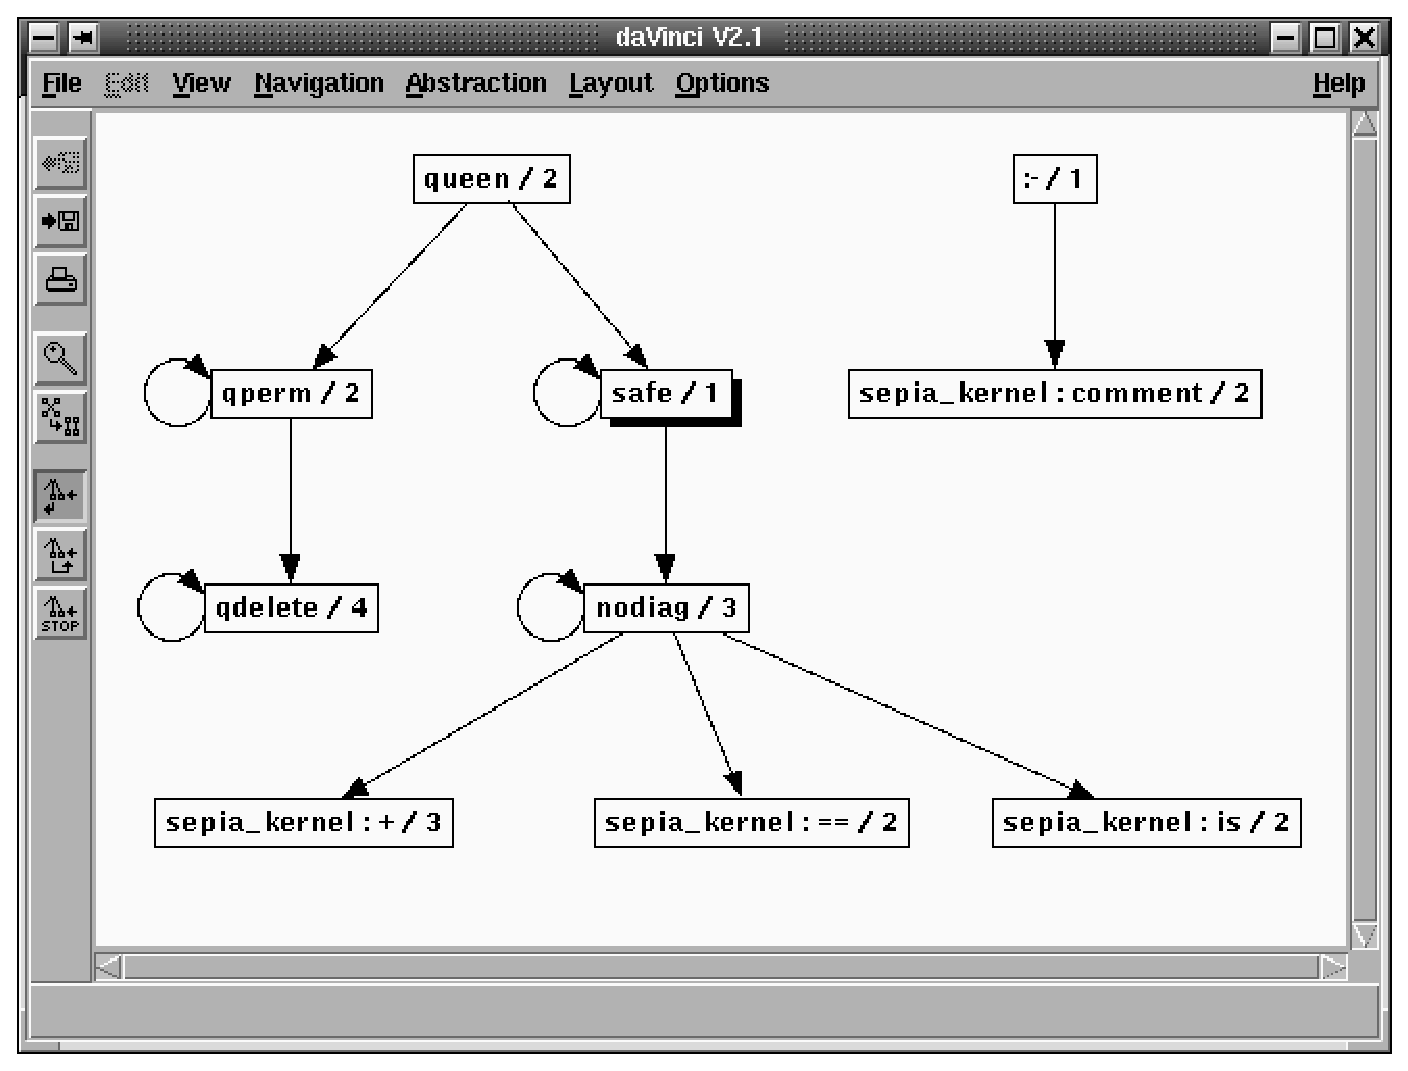
\includegraphics{xrefDavinci.eps}}
\end{center}
\caption{Call graph for queen example with built-in predicates}
\label{xrefdavinci}
\end{figure}

%----------------------------------------------------------------------
\section{Pretty Printer Tool}
%----------------------------------------------------------------------

The pretty printer library provides a set of predicates for the printing
of a file's contents as a file in a number of formats.
In particular, an {\eclipse} source file can be converted into an
HTML document with proper indentation, syntax colouring, hyperlinks
from predicate uses to definition, and hyperlinks to documentation.

The \bipref{pretty_print/2}{../bips/lib/pretty_printer/pretty_print-2.html}
predicate is used to print the file, or list of files.
A list of options can be given which modifies the format of the output
file, its location, etc.  The following creates subdirectory \notation{pretty}
in the current directory. Within the \notation{pretty} directory reside
\notation{index.html} and \notation{queen.html}, where \notation{queen.html} is
the \notation{queen} module pretty printed in HTML:

\begin{quote}
\begin{verbatim}
?- pretty_printer:pretty_print(queen).
Writing /examples/pretty/queen.html
\end{verbatim}
\end{quote}

\vfill %<<<<<<<<<<<<<<<<<<<<<<<<<<<<


%----------------------------------------------------------------------
\section{Timing Profiler}
%----------------------------------------------------------------------

The \Index{profiling} tool helps to find \emph{hot spots} in
a program that are worth optimising.
To use the profiler, start \eclipse{} or \tkeclipse{} with the
\notation{-P} command line option (or use the EC_OPTION_WITH_PROFILER
via the C interface, or the with_profiler option via the Tcl interface,
see \ref{cmdlineopts}).
It is not necessary to compile the profiled code in a special way;
this profiler works independently of compiler optimizations and debug mode.

To profile the execution of a particular goal, use
\bipref{profile/1}{../bips/lib/profile/profile-1.html}:
\begin{quote}
\begin{verbatim}
?- profile(Goal).
\end{verbatim}
\end{quote}
or select the \emph{Time Profile} option from \tkeclipse{}'s Query-menu.
The profiler then executes the \about{Goal} in
the profiling mode, which means that every 100th of a second the
execution is interrupted and the profiler records the currently
executing procedure.  For example
\begin{quote}
\begin{verbatim}
?- profile(queen([1,2,3,4,5,6,7,8,9],Out)).
goal succeeded

		  PROFILING STATISTICS
		  --------------------
Goal:             queen([1, 2, 3, 4, 5, 6, 7, 8, 9], Out)
Result:		  success
Sampling rate:	  every 0.01s process_cputime
Samples taken:	  2
Thread cputime:	  0.03s

Predicate             Module        %Time   Time   %Cum
--------------------------------------------------------
qdelete           /4  eclipse       50.0%   0.01s  50.0%
nodiag            /3  eclipse       50.0%   0.01s 100.0%

Out = [1, 3, 6, 8, 2, 4, 9, 7, 5]
Yes (0.14s cpu)
\end{verbatim}
\end{quote}

The profiler output contains the following information:
\begin{enumerate}
\item The line \notation{Goal:} shows the goal which was profiled.
\item The line \notation{Result:} indicates whether the specified goal
\emph{succeeded}, \emph{failed} or \emph{aborted}.  The
\predspec{profile/1} predicate itself always succeeds.
\item The next lines show the sampling rate and the number of samples taken.
\item The next line shows the time spent in the calling thread.
\item Finally the predicates which were being executed when the
profiler sampled, ranked in decreasing sample count order are shown.
\end{enumerate}


Auxiliary system predicates are printed under a
common name without arity, e.g., \notation{arithmetic} or
\notation{all_solutions}.
Predicates which are local to locked modules are printed
together on a single line that contains only the module name.
By default only predicates written in Prolog are profiled, i.e.,
if a Prolog predicate calls an external or built-in predicate
written in C, the time will be assigned to the Prolog predicate.

The predicate \predspec{profile(Goal,~Flags)} can be used to change
the way profiling is made, \about{Flags} is a list of flags.
Currently only the flag \notation{simple} is accepted and it
causes separate profiling of simple predicates, i.e.,
those written in C.

The problem with the results displayed above is that the sampling
frequency is too low when compared to the total user time spent
executing the goal.  In fact in the above example the profiler was
only able to take two samples before the goal terminated.

The frequency at which the profiler samples is fixed, so in order to
obtain more representative results one should have an auxiliary
predicate which calls the goal a number of times, and compile and
profile a call to this auxiliary predicate. e.g.,

\begin{quote}
\begin{verbatim}
queen_100 :-
  (for(_,1,100,1) do queen([1,2,3,4,5,6,7,8,9],_Out)).
\end{verbatim}
\end{quote}

Note that, when compiled, the above \predspec{do/2} loop would be
efficiently implemented and not cause overhead that would distort the
measurement.  Section \ref{doloops} presents a
detailed description of logical loops.

\vfill %<<<<<<<<<<<<<<<<<<<<<<<

\begin{quote}
\begin{verbatim}
?- profile(queen_100).
goal succeeded

		  PROFILING STATISTICS
		  --------------------
Goal:             queen_100
Result:		  success
Sampling rate:	  every 0.01s process_cputime
Samples taken:	  319
Thread cputime:	  3.19

Predicate             Module        %Time   Time   %Cum
--------------------------------------------------------
nodiag            /3  eclipse       52.2%   1.67s  52.2%
qdelete           /4  eclipse       27.4%   0.87s  79.6%
qperm             /2  eclipse       17.0%   0.54s  96.5%
safe              /1  eclipse        2.8%   0.09s  99.4%
queen             /2  eclipse        0.6%   0.02s 100.0%

Yes (3.33s cpu)
\end{verbatim}
\end{quote}

In the above example, the profiler takes over three hundred samples
resulting in a more accurate view of where the time is being spent in
the program.  In this instance we can see that more than half of the
time is spent in the \predspec{nodiag/3} predicate, making it an ideal
candidate for optimisation.  This is left as an exercise for the
reader.

Limitation: in \eclipse{}7.0, only the engine that called profile/1
is profiled.

%----------------------------------------------------------------------
\section{Port Profiler}
%----------------------------------------------------------------------
\libidx{port_profiler}
The port profiler is a performance analysis tool based on the idea of
counting of events during program execution.  The events that are
counted are defined in terms of the ``box model'' of execution (the same
model that the debugger uses, see chapter \ref{boxmodel}).  In this
box model, predicates are entered though \about{call}, \about{redo} or
\about{resume} ports,
and exited through \about{exit}, \about{*exit}, \about{fail} or \about{leave}
ports.  Some other interesting events are indicated by ports as well
(\about{next}, \about{else}, \about{delay}).

The usage is as follows:
\begin{enumerate}
\item Compile your program in debug mode, as you would normally do during
program development.
\item Load the \libspec{port_profiler} library
\item Run the query which you want to examine, using
\predspecidx{port_profile/2}:
\begin{quote}
\begin{verbatim}
?- port_profile(queen([1,2,3,4],Out), []).
\end{verbatim}
\end{quote}
\end{enumerate}
This will print the results in a table like the following:

\vfill %<<<<<<<<<<<<<<<<<<<<<<

\begin{verbatim}
PREDICATE       CALLER               call     exit     fail    *exit     redo
-           /3  nodiag      /3         46       46        .        .        .
=\=         /2  nodiag      /3         46       45        1        .        .
qperm       /2  qperm       /2         30       28        .       16       14
qdelete     /4  qperm       /2         20       18        .       12       10
nodiag      /3  nodiag      /3         17       14        3        .        .
nodiag      /3  safe        /1         17        7       10        .        .
+           /3  nodiag      /3         17       17        .        .        .
qdelete     /4  qdelete     /4         10        9        .        3        2
qperm       /2  queen       /2          1        .        .       11       10
safe        /1  queen       /2         11        1       10        .        .
safe        /1  safe        /1          7        4        3        .        .
queen       /2  trace_body  /2          1        .        .        1        .
\end{verbatim}
Each row of the table shows the information for a particular predicate
(by default split according to different caller predicates).
The table is sorted according to entry port count ($call+redo+resume$).
The port counts give information about:
\begin{itemize}
\item what are the most frequently called predicates (\notation{call} ports);
\item whether predicates failed unexpectedly (\notation{fail} ports);
\item whether predicates exited nondeterministically (\notation{*exit} ports),
  i.e.,
    whether they left behind any choice-points for backtracking;
\item whether nondeterministically exited predicates were ever re-entered
    to find alternative solutions (\notation{redo} ports);
\item whether predicates did internal backtracking (\notation{next} ports) in
  order
    to find the right clause (this may indicate suboptimal indexing);
\item how often predicates were delayed and resumed.
\end{itemize}
For more details about different options and output formats, see
the description of
\biprefni{port_profiler}{../bips/lib/port_profiler/index.html}%
\libidx{port_profiler}
in the \about{Reference Manual}.


%----------------------------------------------------------------------
\section{Line coverage}
%----------------------------------------------------------------------
\libidx{coverage}\index{line coverage}
The line coverage library provides a means to ascertain exactly how
many times individual clauses are called during the evaluation of a
query.

\index{coverage counters}
The library works by placing \emph{coverage counters} at strategic
points throughout the code being analysed.  These counters are
incremented each time the evaluation of a query passes them.  There
are three locations in which coverage counters can be inserted.
\begin{enumerate}
\item At the beginning of a code block.
\item Between predicate calls within a code block.
\item At the end of a code block.
\end{enumerate}
A code block is defined to be a conjunction of predicate calls, i.e., a
sequence of goals separated by commas.

The counter values do not only show whether all code points were
reached but also whether subgoals failed or aborted (in which case
the counter before a subgoal will have a higher value than the
counter after it).

%----------------------------------------------------------------------
\subsection{Compilation}
%----------------------------------------------------------------------
\indextt{ccompile/1}
\index{ccompile!coverage}
In order to add the coverage counters to code, it must be compiled with
the \bipref{ccompile/1}{../bips/lib/coverage/ccompile-1.html}
predicate which can be found in the
\bipref{coverage}{../bips/lib/coverage/index.html} library.

The \predspec{ccompile/1} predicate (note the initial `c' stands for
coverage) can be used in place of the normal \predspec{compile/1}
predicate to compile a file with coverage counters.

The following shows the results of compiling the \examplename{n-queens} example:
\begin{quote}
\begin{verbatim}
?- coverage:ccompile(queen).
queen.ecl  compiled traceable 6016 bytes in 0.01 seconds
coverage: inserted 20 coverage counters into module queen

Yes (0.14s cpu)
\end{verbatim}
\end{quote}

Once compiled, predicates can be called as usual and will (by default)
have no visible side effects. Internally however, the counters will
be incremented as the execution progresses. The following demonstrates
this for a single solution to the \predspec{queen/2} predicate:
\begin{quote}
\begin{verbatim}
?- queen:queen([1,2,3,4,5,6,7,8,9], Out).
\end{verbatim}
\end{quote}
The counter results are retrieved as demonstrated in the subsequent section.
The two argument predicate \predspecidx{ccompile/2}\index{ccompile!coverage}
can take a list of \notation{name:value} pairs
which can be used to control the exact manner in which coverage
counters are inserted. The documentation for the
\bipref{ccompile/2}{../bips/lib/coverage/ccompile-2.html} predicate
provides for a full list of the available flags.

%----------------------------------------------------------------------
\subsection{Results}
%----------------------------------------------------------------------

To generate an HTML file
containing the coverage counter results, the
\bipref{result/1}{../bips/lib/coverage/result-1.html}\index{result!coverage}
predicate is used:
\begin{quote}
\begin{verbatim}
?- coverage:result(queen).
Writing /examples/coverage/queen.html
index.pl   compiled traceable 335304 bytes in 0.17 seconds

Yes (0.18s cpu)
\end{verbatim}
\end{quote}
This creates the result file \notation{coverage/queens.html} which
can be viewed using any browser.  It contains a pretty-printed form of
the source, annotated with the values of the code coverage counters as
described above. As a side effect, the coverage counters will be reset.

%\index{reset_counters/0} \index{reset_counters!coverage} Having
%generated and viewed results for one run, the coverage counters can be
%reset by calling the
%\bipref{reset_counters/0}{../bips/lib/coverage/reset_counters-0.html}
%predicate:
%\begin{quote}
%\begin{verbatim}
%?- coverage:reset_counters.
%
%Yes (0.00s cpu)
%\end{verbatim}
%\end{quote}

%----------------------------------------------------------------------
\section{Mode analysis}
%----------------------------------------------------------------------
The \libspec{mode_analyser} library is a tool that assists in the generation
of the \predspec{mode/1} directive for predicate definitions. This directive
informs
the compiler that the arguments of the specified predicate will always
have the corresponding form when the predicate is called. The compiler
utilises this information during compilation of the predicate in order
to generate more compact and/or faster code. Specifying the mode of a
predicate that has already been compiled has no effect, unless it is
recompiled. If the specified procedure does not exist, a local undefined
procedure is created.

The mode analyser inserts instrumentation into the clause definitions
of predicates during compilation in order to record mode usage of each
predicate argument. The code should then be run (as many times as is
necessary to capture the most common invocations of each predicate
undergoing analysis). Finally, the results of the analysis are requested
and the suggested mode annotations for each predicate are displayed.

The usage is as follows:
\begin{enumerate}
\item Load the \libspec{mode_analyser} library:
\begin{quote}
\begin{verbatim}
?- lib(mode_analyser).
\end{verbatim}
\end{quote}
\item Compile your program with the mode analyser:
\begin{quote}
\begin{verbatim}
?- analyse(queen).
\end{verbatim}
\end{quote}
\item Run the query which most accurately exercises the
invocation modes of the defined predicates:
\begin{quote}
\begin{verbatim}
?- queen:queen([1,2,3,4],Out).
\end{verbatim}
\end{quote}
\item Generate the results for the module into which
the program was compiled:
\begin{quote}
\begin{verbatim}
?- result([verbose:on])@queen.
\end{verbatim}\end{quote}
\end{enumerate}
This will print the results as follows:
\begin{quote}
\begin{verbatim}
Mode analysis for queen : qdelete / 4:
        Results for argument 1:
                -: 23   *: 0    +: 0    ++: 0
        Results for argument 2:
                -: 0    *: 0    +: 0    ++: 23
        Results for argument 3:
                -: 0    *: 0    +: 0    ++: 23
        Results for argument 4:
                -: 0    *: 0    +: 23   ++: 0

        qdelete(-, ++, ++, +)

Mode analysis for queen : nodiag / 3:
        Results for argument 1:
                -: 0    *: 0    +: 0    ++: 62
        Results for argument 2:
                -: 0    *: 0    +: 0    ++: 62
        Results for argument 3:
                -: 0    *: 0    +: 0    ++: 62

        nodiag(++, ++, ++)

Mode analysis for queen : qperm / 2:
        Results for argument 1:
                -: 0    *: 0    +: 0    ++: 41
        Results for argument 2:
                -: 0    *: 0    +: 41   ++: 0

        qperm(++, +)

Mode analysis for queen : queen / 2:
        Results for argument 1:
                -: 0    *: 0    +: 0    ++: 1
        Results for argument 2:
                -: 1    *: 0    +: 0    ++: 0

        queen(++, -)

Mode analysis for queen : safe / 1:
        Results for argument 1:
                -: 0    *: 0    +: 0    ++: 38

        safe(++)
\end{verbatim}
\end{quote}

NOTE: It is imperative to understand that the results of mode analysis
are merely suggestions for the invocation modes of a predicate based on
runtime information. If there are potential predicate invocation modes
that were not exercised during runtime, the tool is unable to account
for them in its analysis. For the mode specifier '-' the mode analyser
does not determine whether the variable occurs in any other argument
(i.e., is aliased), this must be manually verified.
In summary, the programmer must verify that the suggested modes are correct
before using the directive in the code.  If the instantiation of the
predicate call violates its mode declaration, no exception is raised and
its behaviour is undefined.

For more details about invocation mode analysis see
the description of
\biprefni{mode_analyser}{../bips/lib/mode_analyser/index.html}%
\libidx{mode_analyser}
in the \about{Reference Manual}.

%HEVEA\cutend
